\documentclass{article}

\usepackage{qtree}
\usepackage{graphicx}

\begin{document}
\title{Homework 14}
\date{}
\maketitle

% 1. Spring 08 Final, #1a, #1b
% 2. Fall 08 Final, #1a, #1b
% 3. Fall 10 Final, #3a
% 4. Spring 12 final, #3a, #3ab

\paragraph{\Large 1. Spring 2008 Final Questions 2a and 2b}\mbox{}\\
Consider the following weighted graph.\\
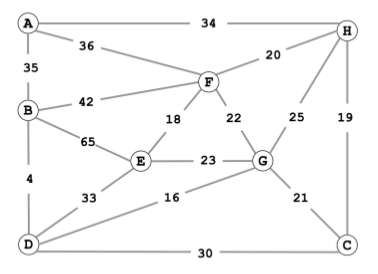
\includegraphics[]{fin-s08-2.png}\\
\begin{enumerate}
\renewcommand{\theenumi}{\Alph{enumi}}
	\item Complete the list of edges in the MST in the order that \textit{Kruskal's algorithm} includes them. For reference, the edge weights in ascending order are:\\
	4  16  18  19  20  21  22  23  25  30  33  34  35  36  42  65\\

	B-D D-G E-F C-H F-H C-G A-H

	\item Complete the list of edges in the MST in the order that \textit{Prim's algorithm} includes them. Start Prim's algorithm from vertex A.\\

	A-H C-H F-H E-F C-G D-G B-D 

\end{enumerate}


\paragraph{\Large 2. Fall 2008 Final Questions 2a and 2b}\mbox{}\\
Consider the following weighted graph with 10 vertices and 21 edges. Note that the edge weights are distinct integers between 1 and 21.\\
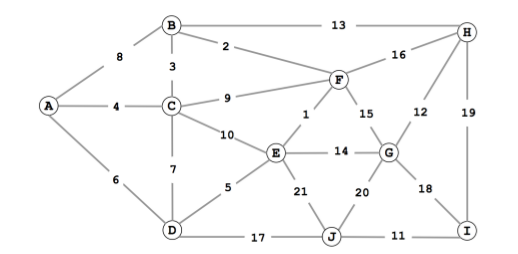
\includegraphics[]{fin-f08-2.png}\\
\begin{enumerate}
\renewcommand{\theenumi}{\Alph{enumi}}
	\item Complete the sequence of edges in the MST in the order that \textit{Kruskal's algorithm} includes them.\\

	1 2 3 4 5 11 12 13 17

	\item Complete the sequence of edges in the MST in the order that \textit{Prim's algorithm} includes them. Start Prim's algorithm from vertex $A$\\

	4 3 2 1 5 13 12 17 11
\end{enumerate}

\paragraph{\Large 3. Study Guide Question}\mbox{}\\
Would Kruskal's or Prim's algorithm work with edge-weighted digraphs?\\

No. It is possible to imagine a scenario in which the edge that either algorithm would pick could not be picked due to the direction of the graph's edges.

\end{document}